\section{Experimental Study}
\label{sec-exp}

In this section, we present an extensive experimental study of our ensemble-enabled approach for link prediction.
Using real-life datasets, we conducted four sets of experiments to evaluate:
(1) the \marked{robustness} and efficiency of our bagging methods with the top-$(\epsilon, k)$ speeding up technique,
node uptake and edge filter techniques (referred to as bagging+ methods)
vs. their counterparts bagging methods with only node uptake technique developed in \cite{liang2016},
(2) the \marked{robustness} and efficiency of our approach vs. conventional methods \Aa \cite{adamic},
\marked{\RA \cite{zhou2009}} and \BIGCLAM \cite{yang-wsdm2013},
and (3) the impacts of various \marked{parameters}.
%and (4) the improvements of bagging+ methods.


\subsection{Experimental settings}

We first present our experimental settings.

\stitle{Real-life datasets}. We used the real-life network datasets
from the Koblenz Network Collection ({\small http://konect.uni-koblenz.de/}).


\begin{enumerate}

\item[(1)] \Digg is a 5 year friendship graph of Digg users with
$279,630$ nodes and $1,731,653$ directed edges.

\item[(2)] \YouTube is a 7 month  friendship graph of YouTube users
with $3,223,589$ nodes and $9,375,374$ undirected edges.

\item[(3)]  \Wikipedia is a 6 year English Wikipedia hyperlink graph
with $1,870,709$ nodes and $39,953,145$ directed edges.

\item[(4)]  \Flickr is a 6 month friendship connections of Flickr users
with $2,302,925$ nodes and $33,140,017$ directed edges.

\item[(5)]  \Twitter is the follower network from Twitter with $41,652,230$ nodes
  and $1,468,365,182$ directed edges.

\item[(6)]  \Friendster is the friendship graph of the Friendster with $68,349,466$
  nodes and $2,586,147,869$ directed edges.

\end{enumerate}


Here (1) \Digg, \YouTube, \Wikipedia and \Flickr contain timestamps of edge arrivals.
For each of these datasets, the latest five month part
is treated as its ground truth data for testing the accuracy,
and the remaining part is treated as its training data,
shown in Table~\ref{tab_dataset}. To test the scalability, we further generated
five subnetworks with increasing sizes for each dataset,
using the breadth first search started from the node with the largest degree.
(2) \Twitter and \Friendster do not have timestamps,
and are only used for the scalability test.
(3) It does not make much sense to predict links for users
who appear in the ground truth data, but not in the training data.
Hence, we removed these users from the ground truth data. Moreover,
since our link prediction methods focus on predicting links on
undirected graphs, we ignored the direction of edges in the directed graphs.




\begin{table}[tb!]
\caption{Training and ground truth data. The data in the first time slot is the training data and
the remaining is the ground truth data.}
\label{tab_dataset}
\vspace{-2ex}
\centering
\begin{tabular}{cccc}
\hline \hline Datasets & Date & Nodes &  Edges  \\
\hline \hline
 & 2005-08-06 --- 2009-02-08 & 207,570 & 1,049,611 \\
\raisebox{1.0ex}[0pt]{ \Digg } & 2009-02-09 --- 2009-07-08 & 207,570 & 467,816 \\
\hline
 & 2006-12-09 --- 2007-02-22 & 1,503,841 & 3,691,893 \\
\raisebox{1.0ex}[0pt]{ \YouTube } & 2007-02-23 --- 2007-07-22 & 1,503,841 & 806,213 \\
\hline
  & 2006-11-01 --- 2006-11-30 & 1,580,291 & 13,341,698 \\
\raisebox{1.0ex}[0pt]{ \Flickr } & 2006-12-01 --- 2007-05-17 & 1,580,291 & 3,942,599 \\
\hline
 & 2001-02-19 --- 2006-10-31 & 1,682,759 & 28,100,011 \\
\raisebox{1.0ex}[0pt]{ \Wikipedia } & 2006-11-01 --- 2007-04-05 & 1,682,759 & 5,856,596\\
\hline \hline
\end{tabular}
\vspace{-2ex}
\end{table}

\begin{table}[tb!]
\caption{Parameters used in the experiments.
Note that we set $k =  10^5$ for \Digg and \YouTube and $k = 10^6$ for
other datasets, respectively.}
\label{tab_parameter}
\vspace{-2ex}
\centering
\newcommand{\tabincell}[2]{\begin{tabular}{@{}#1@{}}#2\end{tabular}}
\begin{tabular}{c l c}
\hline \hline Parameters & Descriptions & Default  \\
\hline \hline
 $\beta$  & Coefficient in \NMF update rule & 0.5\\
 $iter$   & Number of iterations for \NMF   & 50 \\
 $r$      & Number of latent factors       & 10 / 30 \\
\hline
$\epsilon$ & Tolerance of top-($\epsilon$, $k$) prediction & 1 \\
$k$        & \tabincell{l}{Number of links returned by \\ top-($\epsilon$, $k$) prediction} & $10^5 $ / $10^6$   \\
\hline
$\mu$ & \tabincell{l}{Expected appearing times of each \\
node pair in ensemble components} & 0.1 \\
$f$   & \tabincell{l}{Fraction of the number of nodes to be\\
 selected for an ensemble component} & 0.1 \\
$\rho$   &  \tabincell{l}{Fraction of the number of edges to be\\
 selected for an ensemble component} & 0.75 \\
\hline
$n$ & Number of nodes & see Table \ref{tab_dataset}\\
\hline \hline
\end{tabular}
\vspace{-2ex}
\end{table}



\begin{figure*}[tb!]
  \centering
  %\vspace{-2ex}
  % Requires \usepackage{graphicx}
  \subfigure[Digg]{\label{fig_exp_1_1_k_acc_digg}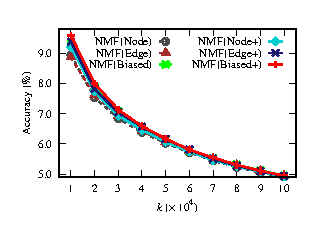
\includegraphics[width= 1.8in, height=1.2in]{eps-script/1-1-a.eps} }
  \quad\quad
  \subfigure[YouTube]{\label{fig_exp_1_1_k_acc_youtube}\includegraphics[width= 1.8in, height=1.2in]{eps-script/1-1-b.eps} }
  \quad\quad
  \subfigure[Wikipedia]{\label{fig_exp_1_1_k_acc_wikipedia}\includegraphics[width= 1.8in, height=1.2in]{eps-script/1-1-c.eps} }
  \subfigure[Digg]{\label{fig_exp_1_1_k_time_digg}\includegraphics[width= 1.8in, height=1.2in]{eps-script/1-1-e.eps} }
  \quad\quad
  \subfigure[YouTube]{\label{fig_exp_1_1_k_time_youtube}\includegraphics[width= 1.8in, height=1.2in]{eps-script/1-1-f.eps} }
  \quad\quad
  \subfigure[Wikipedia]{\label{fig_exp_1_1_k_time_wikipedia}\includegraphics[width= 1.8in, height=1.2in]{eps-script/1-1-g.eps}}
  \vspace{-1ex}
  \caption{Accuracy and efficiency comparison: with respect to the number $k$ of predicted links.}\label{fig_exp_1_1}
  \vspace{-2ex}
\end{figure*}

\begin{figure*}[tb!]
  \centering
  % Requires \usepackage{graphicx}
  \vspace{1ex}
  \subfigure[Digg]{\label{fig_exp_1_2_size_acc_digg}\includegraphics[width= 1.8in, height=1.2in]{eps-script/1-2-a.eps}}
  \hspace{-2ex}
  \subfigure[YouTube]{\label{fig_exp_1_2_size_acc_youtube}\includegraphics[width= 1.8in, height=1.2in]{eps-script/1-2-b.eps}}
  \hspace{-2ex}
  \subfigure[Wikipedia]{\label{fig_exp_1_2_size_acc_wikipedia}\includegraphics[width= 1.8in, height=1.2in]{eps-script/1-2-c.eps}}
  \hspace{-2ex}
  \subfigure[Twitter]{\label{fig_exp_1_2_size_time_twitter}\includegraphics[width= 1.8in, height=1.2in]{eps-script/1-2-i.eps}}
  \subfigure[Digg]{\label{fig_exp_1_2_size_time_digg}\includegraphics[width= 1.8in, height=1.2in]{eps-script/1-2-e.eps}}
   \hspace{-2ex}
  \subfigure[YouTube]{\label{fig_exp_1_2_size_time_youtube}\includegraphics[width= 1.8in, height=1.2in]{eps-script/1-2-f.eps}}
  \hspace{-2ex}
  \subfigure[Wikipedia]{\label{fig_exp_1_2_size_time_wikipedia}\includegraphics[width= 1.8in, height=1.2in]{eps-script/1-2-g.eps}}
  \hspace{-2ex}
  \subfigure[Friendster]{\label{fig_exp_1_2_size_time_friendster}\includegraphics[width= 1.8in, height=1.2in]{eps-script/1-2-j.eps}}
  \vspace{-1ex}
  \caption{Accuracy and efficiency comparison: with respect to the network sizes.}\label{fig_exp_1_2}
  \vspace{-2ex}
\end{figure*}




\stitle{Algorithms for comparison}. We have carefully chosen a couple of algorithms
to compare with our ensemble-enabled approach.


\sstab (1) \Adamic \cite{adamic}: Algorithm \Aa is a popular neighborhood based method that
  produces a score for each link $(u, v)$, defined as below:
  \[ score(u, v) = \sum_{z \in N(u)\cap N(v)}\frac{1}{\log|N(z)|}, \]
  where $N(u)$ is the set of neighbors of node $u$. L\"{u} \cite{linyuan-2011} showed that
  \Aa performs well on a range of networks because it only concerns 2-hop neighbors and
  reduces much of search space. Therefore, we implemented a top-$k$ link prediction
  method by searching the $k$ largest \Aa scoring links. The complexity of this method is
  $O(nd^2\log(k))$, where $d$ is the average degree of networks. Indeed, there is also another popular link
  prediction method \Katz based on the ensemble of all paths \cite{katz-1953}. However, its
  complexity is $O(n^3)$, and does not work on large networks with millions
  of nodes. Thus, we did not choose \Katz for comparison in the experiments.

\marked{\sstab  (2) \Resource \cite{zhou2009}: Algorithm \RA is another
neighborhood based method that assumes the node $u$ can send some resource
to $v$ with their common neighbors playing the role of transmitters. The
\RA score for a link $(u, v)$ is defined as below:
 \[ score(u, v) = \sum_{z \in N(u)\cap N(v)}\frac{1}{|N(z)|}.\]
Note that \RA is very similar to \Aa when $|N(z)|$ is small, but
 great different when $|N(z)|$ is large. Zhou \etal \cite{zhou2009} showed that
 \RA performs better than \Aa in the networks with high average degree since
 \RA punishes high degree common neighbors more heavily.  Therefore,
 we choose it for comparison in the experiments.}

\sstab  (3) \CAMBN \cite{yang-wsdm2013}:
  Yang and Leskovec developed this probabilistic generative model for networks
  based on community affiliations. An ingredient of \BIGCLAM is based on the fact that,
  when people share multiple community affiliations, the links between them stem for
  one dominant reason. This means that the more communities a node pair shares,
  the higher the probability of the  node pair being connected is.
  Let $F$ be a nonnegative matrix where $F_{uc}$ is the degree of the node $u$ belongs to
  the community $c$. Given $F$, the \BIGCLAM generates a network $G(N, A)$ by creating edge
  $(u, v)$ between a pair of nodes $u, v \in N$ with the probability
    \[ p(u, v) = 1 - \exp(-\overline{F_u}\cdot \overline{F_v}), \]
where $\overline{F_u}$ is a weight vector for node $u$. Viewing the probability $p(u, v)$ as
  a score for the link $(u, v)$, it is reasonable to predict links based on \BIGCLAM.
The complexity of  \BIGCLAM is $O(nd(r + d) )$, where $d$ is the average degree of networks.
  In addition, this model is not designed to search the entire space of $O( n^2 )$,
  and we revised it by our top-($\epsilon$, $k$) method to predict links.


\stitle{Implementation}.
We implemented all algorithms including (a) \Aa, \BIGCLAM,
link prediction method in Section 2 (\NMF),
(b) \NMF with random node bagging (\Node), \NMF with  edge bagging (\Edge),
\NMF with biased edge bagging (\Biased), developed in \cite{liang2016}, and (c) their counterparts \Nodep, \Edgep and \Biasedp with the top-$(\epsilon, k)$ speeding up technique in Section~\ref{sec-NMF-topk-optimization} and the edge filter technique in Section~\ref{subsec-lp-char}, using C/C++ with no parallelization.

% \Node with top-$(\epsilon, k)$ speeding up and edge filter (\Nodep),
%\Edge with top-$(\epsilon, k)$ speeding up and edge filter (\Edgep) and
%\Biased with top-$(\epsilon, k)$ speeding up and edge filter (\Biasedp)



All experiments were conducted on a machine with 2 Intel Xeon
E5--2630 2.4GHz CPUs and 64 GB of Memory, running 64 bit
Windows 7 professional system. Each experiment was repeated 5 times,
and the average is reported here.

\subsection{Experimental Results}


We next present our findings. In all the experiments, we fixed $r$ to
$(50, 50, 50)$ (resp. $(10, 40, 50)$) for \NMF (resp. \BIGCLAM) on
\Digg, \YouTube, and \Wikipedia, respectively, by default. For the bagging+ and bagging
methods, we also fixed $r = 30$ on \Digg and $r = 10$ on other datasets by default
(See Exp-3.4 for more details about the setting of $r$).
%\marked{In addition, we fixed $k$ to the same order of magnitude as the number of links
%in the ground truth data for each dataset \cite{yang2015}.}
The other parameters with their descriptions and default values
are presented in Table \ref{tab_parameter}.

\begin{figure*}[tb!]
  \centering
  %\vspace{-2ex}
  % Requires \usepackage{graphicx}
  \subfigure[Digg]{\label{fig_exp_2_1_k_acc_digg}\includegraphics[width= 1.8in, height=1.2in]{eps-script/2-1-a.eps} }
  \quad\quad
  \subfigure[YouTube]{\label{fig_exp_2_1_k_acc_youtube}\includegraphics[width= 1.8in, height=1.2in]{eps-script/2-1-b.eps} }
  \quad\quad
  \subfigure[Wikipedia]{\label{fig_exp_2_1_k_acc_wikipedia}\includegraphics[width= 1.8in, height=1.2in]{eps-script/2-1-c.eps} }
  \subfigure[Digg]{\label{fig_exp_2_1_k_time_digg}\includegraphics[width= 1.8in, height=1.2in]{eps-script/2-1-e.eps} }
  \quad\quad
  \subfigure[YouTube]{\label{fig_exp_2_1_k_time_youtube}\includegraphics[width= 1.8in, height=1.2in]{eps-script/2-1-f.eps} }
  \quad\quad
  \subfigure[Wikipedia]{\label{fig_exp_2_1_k_time_wikipedia}\includegraphics[width= 1.8in, height=1.2in]{eps-script/2-1-g.eps}}
  \vspace{-1ex}
  \caption{Accuracy and efficiency comparison: with respect to the number $k$ of predicted links.}\label{fig_exp_2_1}
  \vspace{-2ex}
\end{figure*}



%%%%%%%%%%%%%%%%%%%%%%%%%%%%%%%%%%%%   2016-06-22 duan begin
\subsubsection{Bagging+ vs. Bagging}
In the first set of test, we evaluated the \marked{robustness} and efficiency of our bagging+ methods
compared with bagging methods. Given one of top-$k$ link prediction methods, denoted by $x$, its \marked{performance}
of link prediction is evaluated with the following measure:
\begin{equation}
accuracy(x) = \frac{\# \textrm{ of correctly predicted links}}{\textrm{the number} \ k\ \textrm{of predicted links}}.
\end{equation}


We first evaluate the improvements of our bagging+ methods and then
evaluate the impacts of $k$ and network sizes.
Compared with their counterparts bagging methods~\cite{liang2016}, the bagging+ methods have two modifications:
the top-$(\epsilon, k)$ speeding up technique (denoted as top-$(\epsilon, k)$+) and the edge filter technique.
These techniques have no side effects on accuracy.
Therefore, we focus on the efficiency improvements of these techniques.


\stitle{Exp-1.1: Improvements of bagging+ methods}. To evaluate the
efficiency improvements of these techniques, we generated different combinations
of these techniques and fixed the parameters to their default values.
The results of running time are reported in Table \ref{tab_improvements}.

The results tell us that (a) Top-$(\epsilon, k)$+ indeed improves
the efficiency of Top-$k$ on all datasets,
(b) the edge filter technique also speeds up the bagging methods,
and (c) the maximum speedup is obtained by taking the
two techniques together. Therefore, we adopt these two techniques
in our bagging+ methods to achieve the maximum speedup.
Note that the running time of \Biasedp and \Nodep on \YouTube and \Wikipedia
are very close because \Biasedp spends more time on sampling the nodes
from the input graph than \Nodep while \Nodep spends more time on processing
its ensembles. Furthermore, the improvement of Top-$(\epsilon, k)$+ on \Wikipedia is not
distinct since the $\epsilon = 1$ is very suitable for this dataset.

\begin{table}
\caption{Running time (sec.) of different combinations of the modifications. Node+
(resp. Edge+ and Biased+) is the Random Node Bagging (resp. Edge Bagging
and Biased Edge Bagging) with edge filter.}
\label{tab_improvements}
\vspace{-2ex}
\centering
\newcommand{\tabincell}[2]{\begin{tabular}{@{}#1@{}}#2\end{tabular}}
\begin{tabular}{l|l|c|c|c}
\hline \hline Bagging & Top-$k$ Prediction & Digg & YouTube & Wikipedia  \\
\hline \hline
Node & Top-$(\epsilon, k)$           & 74.15    & 43.43 & 134.06  \\
Node & Top-$(\epsilon, k)$+        & 65.01    & 41.29 & 133.80 \\
Node+ & Top-$(\epsilon, k)$        & 67.22    & 40.02 & 118.13  \\
Node+ & Top-$(\epsilon, k)$+    & \textbf{60.38}   & \textbf{37.87} & \textbf{117.27} \\
\hline
Edge & Top-$(\epsilon, k)$            & 77.33   & 47.23 & 137.72  \\
Edge & Top-$(\epsilon, k)$+        & 67.26    & 45.04 & 137.57  \\
Edge+ & Top-$(\epsilon, k)$        & 70.29   & 43.69 & 121.42 \\
Edge+ & Top-$(\epsilon, k)$+    & \textbf{62.31}    & \textbf{41.29} & \textbf{121.16} \\
\hline
Biased & Top-$(\epsilon, k)$         & 63.93    & 42.39 & 135.59  \\
Biased & Top-$(\epsilon, k)$+      & 58.56    & 41.07 & 134.02  \\
Biased+ & Top-$(\epsilon, k)$      & 58.97    & 39.61 & 119.44  \\
Biased+ & Top-$(\epsilon, k)$+  & \textbf{55.32}    & \textbf{38.15} & \textbf{117.25}  \\
\hline \hline
\end{tabular}
\vspace{-2ex}
\end{table}





\stitle{Exp-1.2: Impacts of $k$}. To evaluate the impacts of the number $k$ of
predicted links, we varied $k$ from $1\times 10^4$ to $1\times 10^5$ on \Digg
and \YouTube (resp. from $1\times 10^5$ to $1\times 10^6$ on \Wikipedia)
and fixed other parameters to their default values.
The results of accuracy and running time are reported in Figures \ref{fig_exp_1_1_k_acc_digg}--\ref{fig_exp_1_1_k_acc_wikipedia}
and Figures \ref{fig_exp_1_1_k_time_digg}--\ref{fig_exp_1_1_k_time_wikipedia}, respectively.




The accuracy results tell us that
(a) \Biased and \Biasedp are the best methods on all datasets,
(b) the accuracy of the bagging+ methods are very close to that
of their counterparts bagging methods, and (c) the accuracy of all
methods decreases with the increase of $k$. It is means that the
bagging+ methods maintain the accuracy while some of the
edges have been removed compared with their counterparts bagging methods.
This verifies the \marked{robustness} of the bagging+ methods.


The running time results tell us that (a) the \Biasedp outperforms
other methods on all datasets, (b) the three bagging+ methods are faster
than their counterparts bagging methods, and (c) the running time of all
methods increase slightly with the increase of $k$. For instance,
\Biasedp is $(1.2, 1.1, 1.2)$ times faster than
\Biased on \Digg, \YouTube and \Wikipedia, respectively.
This verifies the efficiency of the bagging+ methods.







\stitle{Exp-1.3: Impacts of network sizes}. To evaluate the impacts of network sizes, we varied the
number of nodes $n$ from $3\times 10^4$ to $1.5\times 10^5$ on \Digg (resp.
from $3\times 10^5$ to $1.5\times 10^6$ on \YouTube and \Wikipedia,
from $3\times 10^5$ to $5\times 10^6$ on \Twitter and
from $1\times 10^6$ to $1.5\times 10^7$ on \Friendster).
Since \Twitter and \Friendster do not contain ground truth for choosing the value of $r$,
we fixed $r$ on these datasets to the average value of
its default values. Hence, on these two datasets, we fixed $r = 50$ for \NMF
(resp. $r = 33$ for \BIGCLAM and $r = 17$ for the bagging methods). The results
of accuracy and running time are reported in Figures \ref{fig_exp_1_2_size_acc_digg}--\ref{fig_exp_1_2_size_acc_wikipedia}
and Figures \ref{fig_exp_1_2_size_time_twitter}--\ref{fig_exp_1_2_size_time_friendster}, respectively.



The accuracy results tell us that (a) \Biased has the highest accuracy on all
datasets among the three bagging methods, (b) the three bagging+ methods perform as well as their counterparts
bagging methods. This means that the bagging+ methods are also accurate and
robust with the increase of network sizes.

The running time results tell us that (a) \Biasedp is the fastest method on all
datasets, (b) the bagging+ methods are faster than their counterparts bagging
methods, and (c) the running time of all methods increase nearly linearly with the
increase of $n$. For instance, \Biasedp speeds up \Biased for around
$1.3$ (resp. $1.4$) times on \Twitter (resp. \Friendster) and is thus essential for
making our bagging+ methods scale better than their counterparts to large networks.


\eat{Note that the running time of all methods at $n = 5\times 10^6$ on \Twitter
increases rapidly because the average degree is $83$ on this subnetwork while less
than $55$ on other subnetworks. }


\begin{figure*}[tb!]
  \centering
  % Requires \usepackage{graphicx}
  \vspace{1ex}
  \subfigure[Digg]{\label{fig_exp_2_2_size_acc_digg}\includegraphics[width= 1.8in, height=1.2in]{eps-script/2-2-a.eps}}
  \hspace{-2ex}
  \subfigure[YouTube]{\label{fig_exp_2_2_size_acc_youtube}\includegraphics[width= 1.8in, height=1.2in]{eps-script/2-2-b.eps}}
  \hspace{-2ex}
  \subfigure[Wikipedia]{\label{fig_exp_2_2_size_acc_wikipedia}\includegraphics[width= 1.8in, height=1.2in]{eps-script/2-2-c.eps}}
  \hspace{-2ex}
  \subfigure[Twitter]{\label{fig_exp_2_2_size_time_twitter}\includegraphics[width= 1.8in, height=1.2in]{eps-script/2-2-i.eps}}
  %\hspace{-2ex}
  \subfigure[Digg]{\label{fig_exp_2_2_size_time_digg}\includegraphics[width= 1.8in, height=1.2in]{eps-script/2-2-e.eps}}
\hspace{-2ex}
\subfigure[YouTube]{\label{fig_exp_2_2_size_time_youtube}\includegraphics[width= 1.8in, height=1.2in]{eps-script/2-2-f.eps}}
  \hspace{-2ex}
  \subfigure[Wikipedia]{\label{fig_exp_2_2_size_time_wikipedia}\includegraphics[width= 1.8in, height=1.2in]{eps-script/2-2-g.eps}}
  \hspace{-2ex}
  \subfigure[Friendster]{\label{fig_exp_2_2_size_time_friendster}\includegraphics[width= 1.8in, height=1.2in]{eps-script/2-2-j.eps}}
  \vspace{-1ex}
  \caption{Accuracy and efficiency comparison: with respect to the network sizes.}\label{fig_exp_2_2}
  \vspace{-2ex}
\end{figure*}

\begin{figure*}[tb!]
  \centering
  %\vspace{-2ex}
  % Requires \usepackage{graphicx}
  \subfigure[Digg]{\label{fig_exp_3_mu_acc_digg}\includegraphics[width= 1.8in, height=1.2in]{eps-script/3-1-a.eps}}
  \quad\quad
  \subfigure[YouTube]{\label{fig_exp_3_mu_acc_youtube}\includegraphics[width= 1.8in, height=1.2in]{eps-script/3-1-b.eps}}
  \quad\quad
  \subfigure[Wikipedia]{\label{fig_exp_3_mu_acc_wikipedia}\includegraphics[width=1.8in, height=1.2in]{eps-script/3-1-c.eps}}
  \subfigure[Digg]{\label{fig_exp_3_mu_time_digg}\includegraphics[width=1.8in, height=1.2in]{eps-script/3-1-e.eps}}
  \quad\quad
  \subfigure[YouTube]{\label{fig_exp_3_mu_time_youtube}\includegraphics[width=1.8in, height=1.2in]{eps-script/3-1-f.eps}}
  \quad\quad
  \subfigure[Wikipedia]{\label{fig_exp_3_mu_time_wikipedia}\includegraphics[width=1.8in, height=1.2in]{eps-script/3-1-g.eps}}
  \vspace{-1ex}
  \caption{Accuracy and efficiency comparison: with respect to the expected appearing times $\mu$.}\label{fig_exp_3_mu}
  \vspace{-2ex}
\end{figure*}


\begin{table}
\caption{Accuracy (\%) comparison with \Aa, \RA and \BIGCLAM.}
\label{tab_accuracy}
\vspace{-2ex}
\centering
\newcommand{\tabincell}[2]{\begin{tabular}{@{}#1@{}}#2\end{tabular}}
\begin{tabular}{l|c|c|c}
\hline \hline Algorithm  & Digg & YouTube & Wikipedia  \\
\hline \hline
\Aa & 3.50 &	1.57 &	2.14  \\
\RA & 2.32 &	1.65 &	\textbf{3.09}  \\
\BIGCLAM & 3.70 $\pm$ (0.256) &	1.56 $\pm$ (0.190) &	1.82 $\pm$ (0.100)  \\
\NMF & 4.83 $\pm$ (0.072) 	&2.12 $\pm$ (0.090) 	&2.05 $\pm$ (0.109) \\
\Biased & \textbf{4.95 $\pm$ (0.076)}	& \textbf{2.28 $\pm$ (0.159)}	& 2.31 $\pm$ (0.038) \\
\Biasedp & 4.95 $\pm$ (0.096)	& 2.25 $\pm$ (0.112)	& 2.33 $\pm$ (0.045) \\
\hline \hline
\end{tabular}
\vspace{-2ex}
\end{table}

\subsubsection{Comparison with \Aa, \marked{\RA} and \BIGCLAM}
In the second set of tests, we evaluated the \marked{robustness} and efficiency of our
methods compared with \Aa, \marked{\RA} and \BIGCLAM. From the previous tests, we find that the
\Biasedp and its counterpart \Biased are the best bagging methods. Therefore, we
chose them for the comparison in this set of tests.


\stitle{Exp-2.1: Impacts of $k$}. Using the same setting as Exp-1.2, we evaluated
the impacts of the number $k$ of predicted links.
The results of accuracy and running time are reported in Figures \ref{fig_exp_2_1_k_acc_digg}--\ref{fig_exp_2_1_k_acc_wikipedia}
and Figures \ref{fig_exp_2_1_k_time_digg}--\ref{fig_exp_2_1_k_time_wikipedia}, respectively.
\marked{Moreover, the comparison of accuracy together with its 95\% confidence intervals
when $k$ is fixed to its default value is shown in Table \ref{tab_accuracy}.}

The accuracy results tell us that (a) \Biased outperforms other methods on
\marked{most of the datasets}, (b) the accuracy of \Biasedp is very close to that of \Biased, (c) both
\Biased and \Biasedp have a higher accuracy than \Aa, \marked{\RA and \BIGCLAM, except for \RA on \Wikipedia},
(d) \NMF is more accurate than \marked{\Aa, \RA and \BIGCLAM, except for \RA on \Wikipedia},
and (e) the accuracy of all methods decreases with the increase of $k$.
Indeed, \Biased improves the accuracy by $(2.5\%, 41.4\%, 113.4\%, 34.1\%)$ (resp. $(7.5\%, 45.2\%,$ $ 38.2\%, 46.2\%)$
and $(12.7\%, 7.9\%, -25.2\%, 26.9\%)$) over \NMF, \Aa, \RA and \BIGCLAM on \Digg, \YouTube and \Wikipedia,
respectively. \marked{Moreover, \Biased performs consistently well on all networks (\ie more robust), unlike \RA which works well
on \Wikipedia but poorly on other datasets. This verifies the robustness of our bagging methods.}


The running time results tell us that (a) \Biasedp is the fastest method on all
datasets except \Aa \marked{and \RA are the two fastest} on \Digg since the size of this network is so
small, (b) the two bagging methods are much faster than \NMF, \Aa, \marked{\RA} and \BIGCLAM,
(c) the running time of all methods is insensitive to the increase of $k$,
except \Aa \marked{and \RA} whose complexity is $O(nd^2\log(k))$.
Indeed, the bagging+ and bagging methods finished the prediction in 140 seconds on the three datasets.
Furthermore, \Biasedp is $(7.3, 0.2, 0.1, 1.2)$ (resp. $(90, 1.3, 1.0, 15.5)$ and $(37, 22, 17, 49)$)
times faster than \NMF, \Aa, \marked{\RA} and \BIGCLAM on
\Digg, \YouTube and \Wikipedia, respectively.
This verifies the efficiency of our bagging methods.


Note that the accuracy of all methods is not very high, even the best
accuracy (\Biasedp on \Digg when $k = 1\times 10^4$) is less than $10\%$. The reason is that
there are more than $1\times 10^{10}$ possible links in the search space of each dataset,
but less than $1\times 10^6$ links in the ground truth.
\marked{Since \RA is suitable for high average degree networks \cite{zhou2009},
it performs best on \Wikipedia which has the largest average degree.}
In addition, \NMF is slower than \marked{\Aa and \RA} on three datasets because $r$ is fixed to $50$,
which is consistent to the $O(nr^2)$ complexity of \NMF.
The running time of \marked{\Aa (resp. \RA) is about 50 (resp. 37) seconds on \YouTube,
while more than 2,500 (resp. 1,900) seconds} on \Wikipedia.
This is because that the average degrees of these datasets are 5 and 33,
and \Aa  \marked{and \RA} take more time with the increase of the network degree.

The running time of \BIGCLAM is also sensitive to the degree of networks because its complexity is $O(nd(r + d))$.
As a result, it runs faster than
\NMF on \YouTube when the degree is 5, but takes more time on \Wikipedia
when the degree is increased.








\stitle{Exp-2.2: Impacts of network sizes}. Using the same setting as Exp-1.3, we
evaluated the impacts of network sizes. The results of accuracy and running time
are reported in Figures \ref{fig_exp_2_2_size_acc_digg}--\ref{fig_exp_2_2_size_acc_wikipedia}
and Figures \ref{fig_exp_2_2_size_time_twitter}--\ref{fig_exp_2_2_size_time_friendster}, respectively.
Note that there are {\em some missing plots} for \NMF, \Aa, \marked{\RA} and
\BIGCLAM in the Figures \ref{fig_exp_2_2_size_time_twitter} and
\ref{fig_exp_2_2_size_time_friendster} as they could not finished in 24 hours.



The accuracy results tell us that (a) \Biased obtains the highest accuracy on
\marked{most of the datasets}, (b) \Biasedp performs as well as its counterpart \Biased,
(c) the bagging+ and bagging methods perform better than \NMF, \Aa, \marked{\RA
and \BIGCLAM, except for \RA on \Wikipedia},
and (d) \NMF has a higher accuracy than \Aa, \marked{\RA
and \BIGCLAM, except for \RA on \Wikipedia}. This means that
our methods are more accurate and robust with the increase of network sizes.

The running time results tell us that (a) our bagging+ and bagging methods are much faster than the other methods,
(b) the running time of all methods increase with the increase of $n$. For
instance, \marked{\Biasedp speeds up \NMF, \Aa, \RA and \BIGCLAM for around $(12, 135, 66, 53)$ (resp. $(15, 8, 8, 65)$) }
times on \Twitter (resp. \Friendster) and is thus essential for
making our bagging methods scalable to large networks. Note
that \NMF is slower than \BIGCLAM on \Digg and \YouTube,
but faster on other datasets because \BIGCLAM needs more time with
the increase of the network degree, which is consistent with the complexity analysis.



\begin{figure*}[tb!]
  \centering
  \vspace{1ex}
  % Requires \usepackage{graphicx}
  \subfigure[Digg]{\label{fig_exp_3_f_acc_digg}\includegraphics[width= 1.8in, height=1.2in]{eps-script/3-2-a.eps} }
  \quad\quad
  \subfigure[YouTube]{\label{fig_exp_3_f_acc_youtube}\includegraphics[width= 1.8in, height=1.2in]{eps-script/3-2-b.eps} }
  \quad\quad
  \subfigure[Wikipedia]{\label{fig_exp_3_f_acc_wikipedia}\includegraphics[width= 1.8in, height=1.2in]{eps-script/3-2-c.eps} }
  \subfigure[Digg]{\label{fig_exp_3_f_time_digg}\includegraphics[width= 1.8in, height=1.2in]{eps-script/3-2-e.eps} }
  \quad\quad
  \subfigure[YouTube]{\label{fig_exp_3_f_time_youtube}\includegraphics[width= 1.8in, height=1.2in]{eps-script/3-2-f.eps} }
  \quad\quad
  \subfigure[Wikipedia]{\label{fig_exp_3_f_time_wikipedia}\includegraphics[width= 1.8in, height=1.2in]{eps-script/3-2-g.eps}}
  \vspace{-1ex}
  \caption{Accuracy and efficiency comparison: with respect to the fraction $f$}\label{fig_exp_3_f}
  \vspace{-2ex}
\end{figure*}


\begin{figure*}[tb!]
  \centering
  \vspace{1ex}
  % Requires \usepackage{graphicx}
  \subfigure[Digg]{\label{fig_exp_3_rho_acc_digg}\includegraphics[width= 1.8in, height=1.2in]{eps-script/3-3-a.eps} }
  \quad\quad
  \subfigure[YouTube]{\label{fig_exp_3_rho_acc_youtube}\includegraphics[width= 1.8in, height=1.2in]{eps-script/3-3-b.eps} }
  \quad\quad
  \subfigure[Wikipedia]{\label{fig_exp_3_rho_acc_wikipedia}\includegraphics[width= 1.8in, height=1.2in]{eps-script/3-3-c.eps} }
  \subfigure[Digg]{\label{fig_exp_3_rho_time_digg}\includegraphics[width= 1.8in, height=1.2in]{eps-script/3-3-e.eps} }
  \quad\quad
  \subfigure[YouTube]{\label{fig_exp_3_rho_time_youtube}\includegraphics[width= 1.8in, height=1.2in]{eps-script/3-3-f.eps} }
  \quad\quad
  \subfigure[Wikipedia]{\label{fig_exp_3_rho_time_wikipedia}\includegraphics[width= 1.8in, height=1.2in]{eps-script/3-3-g.eps}}
  \vspace{-1ex}
  \caption{Accuracy and efficiency comparison: with respect to the fraction $\rho$}\label{fig_exp_3_rho}
  \vspace{-2ex}
\end{figure*}



\subsubsection{Impacts of Parameters}
In the third set of tests, we evaluated the impacts of parameters on
the accuracy and running time of bagging+, bagging, \NMF
and \BIGCLAM. We first tested the impacts of $\mu$ and $f$ in bagging+ and bagging methods.
We then tested the impacts of $\rho$ in bagging+ methods. We finally
tested the impacts of $r$ and $\epsilon$.


\stitle{Exp-3.1: Impacts of $\mu$}. To evaluate the impacts of $\mu$, we
varied $\mu$ from $0.01$ to $0.25$ and fixed other parameters to their
default values. The accuracy and running time results are reported in
Figures \ref{fig_exp_3_mu_acc_digg}--\ref{fig_exp_3_mu_acc_wikipedia} and Figures \ref{fig_exp_3_mu_time_digg}--\ref{fig_exp_3_mu_time_wikipedia},
respectively. We also plotted the accuracy and running time of \NMF for comparison.



The results tell us that (a) bagging+ and bagging methods are more accurate than
\NMF when $\mu$ is large enough, (b) the accuracy of bagging+ and bagging methods
increases with the increase of $\mu$ and becomes stable when $\mu$ is greater
than $0.1$. This means that the accuracy of bagging+ and bagging methods would
increase and become stable with the increase of the number of ensemble components.
Furthermore, (c) the running time of bagging+ and bagging methods increases linearly
with the increase of $\mu$ since $\mu / f^2$ ensemble components had been generated in each bagging
method. Note that, when $\mu = 0.1$, the accuracy of bagging+ and bagging methods
is becoming stable and the running time of them is less than \NMF.
Therefore, we fixed $\mu = 0.1$ by default.






\begin{figure*}[tb!]
  \centering
  \vspace{1ex}
  % Requires \usepackage{graphicx}
  \subfigure[Digg]{\label{fig_exp_3_r_acc_digg}\includegraphics[width= 1.8in, height=1.2in]{eps-script/3-4-a.eps} }
  \quad\quad
  \subfigure[YouTube]{\label{fig_exp_3_r_acc_youtube}\includegraphics[width= 1.8in, height=1.2in]{eps-script/3-4-b.eps} }
  \quad\quad
  \subfigure[Wikipedia]{\label{fig_exp_3_r_acc_wikipedia}\includegraphics[width= 1.8in, height=1.2in]{eps-script/3-4-c.eps} }
  \subfigure[Digg]{\label{fig_exp_3_r_time_digg}\includegraphics[width= 1.8in, height=1.2in]{eps-script/3-4-e.eps} }
  \quad\quad
  \subfigure[YouTube]{\label{fig_exp_3_r_time_youtube}\includegraphics[width= 1.8in, height=1.2in]{eps-script/3-4-f.eps} }
  \quad\quad
  \subfigure[Wikipedia]{\label{fig_exp_3_r_time_wikipedia}\includegraphics[width= 1.8in, height=1.2in]{eps-script/3-4-g.eps}}
  \vspace{-1ex}
  \caption{Accuracy and efficiency comparison: with respect to the number $r$ of latent factors.}\label{fig_exp_3_r}
  \vspace{-2ex}
\end{figure*}
\begin{figure*}[tb!]
  \centering
  \vspace{1ex}
  % Requires \usepackage{graphicx}
  \subfigure[Digg]{\label{fig_exp_3_e_acc_digg}\includegraphics[width= 1.8in, height=1.2in]{eps-script/3-5-a.eps} }
  \quad\quad
  \subfigure[YouTube]{\label{fig_exp_3_e_acc_youtube}\includegraphics[width= 1.8in, height=1.2in]{eps-script/3-5-b.eps} }
  \quad\quad
  \subfigure[Wikipedia]{\label{fig_exp_3_e_acc_wikipedia}\includegraphics[width= 1.8in, height=1.2in]{eps-script/3-5-c.eps} }
  \subfigure[Digg]{\label{fig_exp_3_e_time_digg}\includegraphics[width= 1.8in, height=1.2in]{eps-script/3-5-e.eps} }
  \quad\quad
  \subfigure[YouTube]{\label{fig_exp_3_e_time_youtube}\includegraphics[width= 1.8in, height=1.2in]{eps-script/3-5-f.eps} }
  \quad\quad
  \subfigure[Wikipedia]{\label{fig_exp_3_e_time_wikipedia}\includegraphics[width= 1.8in, height=1.2in]{eps-script/3-5-g.eps}}
  \vspace{-1ex}
  \caption{Accuracy and efficiency comparison: with respect to the tolerant $\epsilon$ of top-($\epsilon, k$) prediction.}\label{fig_exp_3_e}
  \vspace{-2ex}
\end{figure*}



\stitle{Exp-3.2: Impacts of $f$}. To evaluate the impacts of $f$, we
varied $f$ from $0.02$ to $0.5$ and fixed other parameters to their
default values. The accuracy and running time results are reported in
Figures \ref{fig_exp_3_f_acc_digg}--\ref{fig_exp_3_f_acc_wikipedia} and
Figures \ref{fig_exp_3_f_time_digg}--\ref{fig_exp_3_f_time_wikipedia}, respectively.



The results tell us that (a) bagging+ and bagging methods have a higher accuracy
than \NMF when $f = 0.1$, (b) the accuracy of bagging methods decreases
with the increase of $f$ when $f$ is greater than 0.1 on \Digg and \Wikipedia,
and (c) the running time of bagging methods increases
nearly linearly with the decrease of $f$. Note that the complexity of bagging methods is
$O((n_{1}r^2 + n_{1}d_{1}r)*\mu /f^2)$, where $n_1 = nf$ and $d_1$ is the average degree of
each ensemble component. Since bagging methods are likely to select dense components, $d_1$
may be greater than $r$ and the complexity is $O(nd_1r\mu /f)$. Thus, the running time
of bagging methods increases with the decrease of $f$. We fixed $f = 0.1$ to keep the accuracy of bagging+ and bagging
methods better than that of \NMF, , by default to achieve a better efficiency.




\stitle{Exp-3.3: Impacts of $\rho$}. To evaluate the impacts of $\rho$ for
the bagging+ methods, we varied $\rho$ from $0.55$ to $0.95$ and
fixed other parameters to their default values. The accuracy and
running time results are reported in
Figures \ref{fig_exp_3_rho_acc_digg}--\ref{fig_exp_3_rho_acc_wikipedia} and
Figures \ref{fig_exp_3_rho_time_digg}--\ref{fig_exp_3_rho_time_wikipedia}, respectively.
We also plotted the accuracy and running time of their counterparts
bagging methods for comparison.

The results tell us that (a) the three bagging+ methods perform
as well as their counterparts bagging methods in accuracy when
$\rho$ is greater than 0.75, (b) the accuracy of the bagging+ methods
increases with the increase of $\rho$, (c) the bagging+ methods are faster
than their counterparts bagging methods when $\rho$ is less than 0.95,
and (d) the running time of the bagging+ methods increases linearly
with the increase of $\rho$, which is consistent with
the complexity that is proportional to the number of edges in the
ensemble component. Keeping the accuracy of the bagging+ methods is close to
that of the bagging methods, we fixed $\rho = 0.75$ by default to achieve a better efficiency.



\stitle{Exp-3.4: Impacts of $r$}. To evaluate the impacts of $r$, we
varied $r$ from $10$ to $50$ and fixed other parameters to their
default values. The accuracy and running time results are reported in
Figures \ref{fig_exp_3_r_acc_digg}--\ref{fig_exp_3_r_acc_wikipedia} and
Figures \ref{fig_exp_3_r_time_digg}--\ref{fig_exp_3_r_time_wikipedia}, respectively.


The results tell us that (a) \Biasedp and \Biased obtain the best accuracy
compared with other methods, (b) bagging+ and bagging methods have a higher accuracy
than \BIGCLAM, (c) the accuracy of \NMF increases slightly with the increase of $r$ and is always
greater than that of \BIGCLAM, and (d) the running time of \NMF is increased
quadratically with the increase of $r$ since its complexity is $O(nr^2)$.
A similar trend of running time is also found for bagging+ and bagging methods.
To obtain the highest accuracy, we fixed $r$ to $(50, 50, 50)$ (resp. $(10, 40, 50)$)
for \NMF (resp. \BIGCLAM) on \Digg, \YouTube and \Wikipedia, respectively.
Note that, when $r = 30$ on \Digg and $r = 10$ on other datasets, the accuracy
of bagging+ and bagging methods is greater than the best accuracy of \NMF. Hence, we
fixed $r = 30$ on \Digg and $r = 10$ on other datasets by default for bagging+ and bagging methods.






\stitle{Exp-3.5: Impacts of $\epsilon$}. To evaluate the impacts of $\epsilon$, we
varied $\epsilon$ from $0.5$ to $1.0$ and fixed other parameters to their
default values. The accuracy and running time results are reported in
Figures \ref{fig_exp_3_e_acc_digg}--\ref{fig_exp_3_e_acc_wikipedia} and
Figures \ref{fig_exp_3_e_time_digg}--\ref{fig_exp_3_e_time_wikipedia}, respectively.



The results tell us that (a) the accuracy of all methods is stable with
the increase of $\epsilon$, which means that the accuracy of our methods is insensitive
to $\epsilon$, and (b) the running time of all methods is decreased with the increase of $\epsilon$
because the larger $\epsilon$ reduces more search space. Thus, our top-($\epsilon$, $k$)
method is reasonable for link prediction. Since the accuracy is insensitive to $\epsilon$, we
fixed $\epsilon = 1$ by default to achieve a better efficiency.




%
%\subsubsection{Performance Improvements of Bagging+ Methods}
%In the fourth set of tests, we evaluate the improvements of our bagging+ methods.
%Compared with their counterparts bagging methods~\cite{liang2016}, the bagging+ methods have two modifications:
%the top-$(\epsilon, k)$ speeding up technique (denoted as top-$(\epsilon, k)$+) and the edge filter technique.
%As shown in previous experiments, these techniques have no side effects on accuracy.
%Therefore, we focus on the efficiency improvements of these techniques.
%
%
%\stitle{Exp-4: Improvements of bagging+ methods}. To evaluate the
%efficiency improvements of these techniques, we generated different combinations
%of these techniques and fixed the parameters to their default values.
%The results of running time are reported in Table \ref{tab_improvements}.
%
%The results tell us that (a) Top-$(\epsilon, k)$+ indeed improves
%the efficiency of Top-$k$ on all datasets,
%(b) the edge filter technique also speeds up the bagging methods,
%and (c) the maximum speedup is obtained by taking the
%two techniques together. Therefore, we adopt these two techniques
%in our bagging+ methods to achieve the maximum speedup.
%Note that the running time of \Biasedp and \Nodep on \YouTube and \Wikipedia
%are very close because \Biasedp spends more time on sampling the nodes
%from the input graph than \Nodep while \Nodep spends more time on processing
%its ensembles. Furthermore, the improvement of Top-$(\epsilon, k)$+ on \Wikipedia is not
%distinct since the $\epsilon = 1$ is very suitable for this dataset.
%
%\begin{table}
%\caption{Running time of different combinations of the modifications. Node+
%(resp. Edge+ and Biased+) is the Random Node Bagging (resp. Edge Bagging
%and Biased Edge Bagging) with edge filter.}
%\label{tab_improvements}
%\vspace{0ex}
%\centering
%\newcommand{\tabincell}[2]{\begin{tabular}{@{}#1@{}}#2\end{tabular}}
%\begin{tabular}{l|l|c|c|c}
%\hline \hline Bagging & Top-$k$ Prediction & Digg & YouTube & Wikipedia  \\
%\hline \hline
%Node & Top-$(\epsilon, k)$           & 74.15    & 43.43 & 134.06  \\
%Node & Top-$(\epsilon, k)$+        & 65.01    & 41.29 & 133.80 \\
%Node+ & Top-$(\epsilon, k)$        & 67.22    & 40.02 & 118.13  \\
%Node+ & Top-$(\epsilon, k)$+    & \textbf{60.38}   & \textbf{37.87} & \textbf{117.27} \\
%\hline
%Edge & Top-$(\epsilon, k)$            & 77.33   & 47.23 & 137.72  \\
%Edge & Top-$(\epsilon, k)$+        & 67.26    & 45.04 & 137.57  \\
%Edge+ & Top-$(\epsilon, k)$        & 70.29   & 43.69 & 121.42 \\
%Edge+ & Top-$(\epsilon, k)$+    & \textbf{62.31}    & \textbf{41.29} & \textbf{121.16} \\
%\hline
%Biased & Top-$(\epsilon, k)$         & 63.93    & 42.39 & 135.59  \\
%Biased & Top-$(\epsilon, k)$+      & 58.56    & 41.07 & 134.02  \\
%Biased+ & Top-$(\epsilon, k)$      & 58.97    & 39.61 & 119.44  \\
%Biased+ & Top-$(\epsilon, k)$+  & \textbf{55.32}    & \textbf{38.15} & \textbf{117.25}  \\
%\hline \hline
%\end{tabular}
%\vspace{-0ex}
%\end{table}



\subsubsection{Analysis of Limitations}
\label{subsction-exp-limit}
\marked{In the last set of tests, we discuss the accuracy limitations of our methods: 
(1) bagging methods might not as good as \NMF in certain situations, and (2) both bagging methods 
and \NMF cannot successfully predict links with large hop distances as well as short distances. 
We first report the accuracy comparison between our bagging methods and \NMF on \Flickr and explain 
the reasons. We then study the accuracy of the bagging methods and \NMF in each hop distance. 
These could be useful when users are to apply our bagging methods in practice.}

%In the last set of tests, we discuss the accuracy limitations of our bagging methods
%compared with \NMF.  Our bagging methods might not as good as \NMF in certain situations.
%We first report the accuracy results of our bagging methods  and  \NMF on \Flickr.
%We then explain the reasons, which could be useful when users are to apply our bagging
%methods in practice.

\begin{figure}[tb!]
  \centering
  %\vspace{1ex}
  % Requires \usepackage{graphicx}
  \subfigure[]{\label{fig_exp_3_r_acc_flickr}\includegraphics[width= 1.7in, height=1.2in]{eps-script/3-4-d.eps} }
  \hspace{-2ex}
  \subfigure[]{\label{fig_exp_2_k_acc_flickr}\includegraphics[width= 1.7in, height=1.2in]{eps-script/2-1-d.eps} }
  \vspace{-1ex}
  \caption{Accuracy comparison on \Flickr: (a) with respect to the number $r$ of latent factors,
  (b) with respect to the number $k$ of predicted links.}\label{fig_exp_5}
  \vspace{-1ex}
\end{figure}

We first report the results on the impact of parameters $r$ and $k$
in Figures \ref{fig_exp_3_r_acc_flickr} and \ref{fig_exp_2_k_acc_flickr}.
We varied $r$ from 10 to 50 (resp. $k$ from $10^5$ to $10^6$)
and fixed other parameters to their default values. The results tell us that
the accuracy of our bagging methods is slightly lower than that of \NMF.
Indeed, \Biased decreases the accuracy by $4\%$ on \Flickr compared with \NMF.

We next explain the reasons. It is well known that the principle in ensemble methods is to make each ensemble as
unique as possible and this is also called as diversity \cite{zhzhou}. Diversity can
be achieved by using different ensemble components or different settings of parameters for the ensemble base
algorithms. Since the base algorithm and its parameters were fixed in our experiments, we examined
the diversity of ensembles generated by our bagging methods. We adopted the pairwise
overlapping of predicted links and nodes (\ie $N_s$ in each ensemble component)
among ensemble components to measure the diversity. The value of pairwise overlapping is between
zero and one and the higher the value means the lower the diversity.
The results are shown in Table \ref{tab_limitations}.

The results tell us that (a) the pairwise overlapping of predicted links on \Flickr is
obviously higher than that on other datasets, which means that the diversity on \Flickr is the
worst one, (b) the pairwise overlapping of nodes for
\Node and \Edge methods on \Flickr is also higher than that on other datasets, which may be
one of reasons decreasing the diversity of these methods. These impair the \marked{performance} of ensemble methods,
which leads to a lower accuracy for our bagging methods on \Flickr than \NMF.

Moreover, observer that \Edge has the highest
pairwise overlapping of predicted links and nodes since this method inclines to select high-degree
nodes repeatedly. Moreover, \Biased overcomes the drawback of \Edge and obtains the lowest pairwise
overlapping, which guarantees its higher accuracy. That is, to gain a high accuracy with the bagging methods, it
is necessary to make each ensemble as unique as possible.


\marked{We also study the distribution of hod distances induced by the links in the ground truth data 
and then compared the accuracy of \BIGCLAM, \NMF and \Biased in each hop distance, shown in Table \ref{tab_hops}. 
Although a large portion of ground truth links are not greater than 3 hops, there are many high-distance links. 
However, \BIGCLAM, \NMF and \Biased are more accurate in predicting 2 or 3 hop links but have little ability to predict 
links with large hop distances. To improve the prediction accuracy, a good predictor should successfully predict 
links in high-distance regions as well as short distance.}

To address these limitations of ensemble-enabled methods, it deserves a full treatment in the future.



\begin{table}
\caption{Pairwise overlapping of predicted links and nodes of ensemble components.}
\label{tab_limitations}
\vspace{-2ex}
\centering
\newcommand{\tabincell}[2]{\begin{tabular}{@{}#1@{}}#2\end{tabular}}
\begin{tabular}{c|l|c|c|c|c}
\hline \hline Overlap & Methods & Digg & YouTube & Wikipedia & Flickr \\
\hline \hline
& Node & 0.57 & 0.54 & 0.39 & \textbf{0.69} \\
& Edge & 0.58 & 0.55 & 0.40 & \textbf{0.72} \\
\raisebox{2.5ex}[0pt]{ Links } & Biased & 0.46 & 0.48 & 0.42 & \textbf{0.67} \\
\hline
& Node & 0.31 & 0.22 & 0.29 & \textbf{0.33} \\
& Edge & 0.35 & 0.27 & 0.30 & \textbf{0.41} \\
\raisebox{2.5ex}[0pt]{ $N_s$ } & Biased & 0.21 & 0.11 & \textbf{0.29} & 0.21 \\
\hline \hline
\end{tabular}
\vspace{-2ex}
\end{table}



\begin{table}
\caption{The distribution of hops between ground truth links and the accuracy 
comparison of \BIGCLAM, \NMF and \Biased in each hop distance.}
\label{tab_hops}
\vspace{-2ex}
\centering
\newcommand{\tabincell}[2]{\begin{tabular}{@{}#1@{}}#2\end{tabular}}
\begin{tabular}{c|c|c|c|c|c|c}
\hline \hline
\multicolumn{4}{c}{The Distribution of Hop Distances} & \multicolumn{3}{|c}{Accuracy of \BIGCLAM} \\
\hline  
Hop  & Digg & YouTube & Wikipedia & Digg & YouTube & Wikipedia \\
\hline 
2 & 32\% & 26\% & 63\%  & 3.8\% & 1.7\% & 1.9\% \\
3 & 39\% & 37\% & 32\%  & 0.4\% & 0.1\% & 0 \\
other & 29\% & 37\% & 5\% & 0 & 0.2\% & 0 \\
\hline \hline  
\multicolumn{4}{c}{Accuracy of \NMF} & \multicolumn{3}{|c}{Accuracy of \Biased}\\
\hline
Hop  & Digg & YouTube & Wikipedia & Digg & YouTube & Wikipedia \\
\hline 
2 & 4.8\% & 2.1\% & 2.1\% & 4.9\% & 2.1\% & 2.4\% \\
3 & 0.8\% & 0.3\% & 2.3\% & 0 & 1.1\% & 0.1\% \\
other & 0 & 0 & 0 & 0 & 0 & 0 \\
\hline \hline
\end{tabular}
\vspace{-2ex}
\end{table}


\stitle{Summary}. From these experimental results on real-life social network datasets,
we find the following.

\sstab (1) \NMF is able to predict links and can be sped up
by the top-($\epsilon$, $k$) process to explore the $O(n^2)$ search space. \NMF is
more accurate than \Aa and \BIGCLAM, which verifies the \marked{robustness}
of \NMF. Moreover, \NMF runs faster than \BIGCLAM on dense networks,
\eg~\Wikipedia, \Twitter and \Friendster, which is consistent with the complexity analysis
that \BIGCLAM is sensitive to the degree of networks.

\sstab (2) The running time of
\NMF, however, is increased quadratically with the increase of $r$. This might be a bottleneck
for large networks. By decomposing the link prediction problem into smaller pieces
and solving them independently, our bagging methods are more efficient and
scale well with the size and density of large networks, especially for the bagging+
methods with the top-$(\epsilon, k)$ speeding up and edge filter techniques,
\eg\ \Biasedp finished in two hours on \Friendster with $1.5\times 10^7$ nodes and
$1.0\times 10^9$ edges, while \NMF, \Aa  and \BIGCLAM could not finish in a day.
Further, \Biasedp speeds up \Biased, \NMF, \Aa and \BIGCLAM
for around $(1.3, 12, 135, 53)$ (resp. $(1.4, 15, 8, 65)$) times on \Twitter (resp. \Friendster).

\sstab (3) Incorporated into link prediction characteristics, our
bagging methods also provide the accuracy advantages for link prediction,
\eg~\Biased improves the accuracy by $(2.5\%$, $41.4\%, 34.1\%)$ (resp. $(7.5\%, 45.2\%, 46.2\%)$ and $(12.7\%, 7.9\%, 26.9\%)$)
over \NMF, \Aa and \BIGCLAM on \Digg, \YouTube and \Wikipedia, respectively.








%%%%%%%%%%%%%%%%%%%%%%%%%%%%%%%%%%%%   2016-06-22 duan end





%
%There are quite a few things that we can show here:
%
%\stitle{Exp-1: Efficiency tests}. We need to show how well our approach
%scales with increasing network size, and the fact that the approach
%remains practically feasible over a much broader range of network
%sizes. So we need some really large real networks, and then by using
%subsets of this network, we can show scalability with increasing
%network size.  A key question here is the choice of baseline to use.
%There are quite a few relevant works belonging to Nitesh Chawla. One
%baseline can of course be our own matrix factorization method
%without the ensembling. But we also need some external and state of
%the art baselines.
%
%
%
%
%\stitle{Exp-2: Accuracy tests}. Ensemble-based methods have the reputation of also
%improving the  accuracy. So it may make sense to check how well the
%approach performs against (i)  the matrix factorization approach
%without ensembling (ii) external baselines.


